\singlespacing

\begin{aufgabe}\label{aufg:formulas}
\TeX en Sie den Text aus \texttt{aufgabe\ref{aufg:formulas}.pdf} so exakt wie m\"oglich nach.	
\end{aufgabe}

\setlength\parindent{18pt} Wenn A und B beliebige Ereignisse sind und $P(B) \leq 0$ ist, dann ist die bedingte Wahrscheinlichkeit von $A$,
vorausgesetzt $B$ (auch die Wahrscheinlichkeit von $A$ unter der Bedingung $B$, notiert als $P(A \mid B)$, definiert
durch:
\begin{displaymath}
 P(A \mid B) = \frac{P(A \cap B)}{P(B)}
\end{displaymath}
Darin ist $P(A \cap B)$ die Wahrscheinlichkeit, dass $A$ und $B$ gemeinsam auftreten. 
$P(A \cap B)$ wird gemeinsame Wahrscheinlichkeit, Verbundwahrscheinlichkeit oder Schnittwahrscheinlicheit genannt.

\newtheorem{mfze}{Theorem}

%\numberwithin{equation}{}
\begin{mfze}{\textbf{Multiplikationssatz für zwei Ereignisse:}}
\begin{equation}
 P(A \cap B) = P(A \mid B) \cdot P(B)
\end{equation}
\end{mfze}

Verallgemeinert man den obigen Ausdruck des Multiplikationssatzes, der für zwei Ereignisse gilt, erhält man den
allgemeinen Multiplikationssatz. Man betrachte dazu den Fall mit $n$ Zufallsereignissen $A_1$ , $A_2$ , $\ldots$ , $A_n$.

\vspace{0.5cm}
\noindent
\begin{equation*}
 \begin{array}{ccccccccc} 
  P\biggl( \bigcap\limits_{i=1}^{n} A_i \biggl) &
  = &
  P(A_1) &
  \cdot &
  \frac{P(A_1 \cap A_2)}{P(A_1)} &
  \cdot &
  \frac{P(A_1 \cap A_2 \cap A_3)}{P(A_1 \cap A_2)} &
  \cdots &
  \frac{P(A_1 \cap A_2 \cap \cdots \cap A_n)}{ P(A_1 \cap A_2) \cap \cdots \cap A_{n-1}) }\\
    &
   = &
   P(A_1) &
   \cdot &
   P(A_2 \mid A_1) &
   \cdot &
   P(A_3 \mid A_1) \cap A_2) &
   \cdots &
   P\Bigl( A_n | \cap_{i=1}^{n-1} A_i \Bigl) \\
 \end{array}
\end{equation*}

\setlength\parindent{18pt} Sind nur bedingte Wahrscheinlichkeiten und die Wahrscheinlichkeiten des bedingenden
Ereignisses bekannt, ergibt sich die totale Wahrscheinlichkeit von A aus

\begin{mfze}{\textbf{Gesetz der totalen Wahrscheinlichkeit:}}
\begin{equation}
 P(A) = P(A \mid B) \cdot P(B) + P(A \mid B^c) \cdot P(B^c),
\end{equation}
\end{mfze}
\noindent \textit{wobei $B^c$ das Gegenereignis zu $B$ bezeichnet.}\\
\\
\indent Wenn $A$ und $B$ stochastisch unabhängig sind, gilt:
\begin{equation*}
 P(A \cap B) = P(A) \cdot P(B),
\end{equation*}
was dann zu Folgendem führt:

\begin{mfze}{\textbf{Stochastische Unabhängigkeit:}}
\\
\textit{Egal, ob das Ereignis $B$ stattgefunden oder nicht stattgefunden hat, ist die Wahrscheinlich-
keit des Ereignisses $A$ stets dieselbe.}
\\
\begin{equation}
\begin{array}{cccclc}
  P(A \mid B) & = & \frac{P(A) \cdot P(B)}{P(B)}  & = & P(A) & \textit{bzw.} \\
  & & &  = &  P(A \mid B^c) & \\
\end{array}
\end{equation}
\end{mfze}

Für den Zusammenhang zwischen $P(A \mid B)$ und $P(B \mid A)$ ergibt sich direkt aus der
Definition und dem Multiplikationssatz:

\newtheorem{cor}[mfze]{Korollar}
\begin{cor}{\textbf{Der Satz von Bayes:}}
 \begin{equation}
  P(A \mid B) = \frac{P(B \mid A) \cdot P(A)}{P(B)}.
 \end{equation}

\noindent \textit{Dabei kann $P(B)$ im Nenner mit Hilfe des Gesetzes der totalen Wahrscheinlichkeit berechnet werden.}
\end{cor}


\begin{aufgabe}
\TeX en Sie folgende Matrix:
\end{aufgabe}

\noindent \underline{Ursprung:} \\
\hspace{1cm} 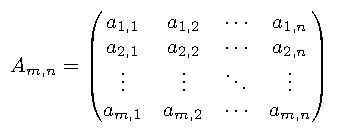
\includegraphics[width=0.4\textwidth]{aufgabe35}

\noindent \underline{nachge\TeX t:}\\ \vspace*{10cm} 
\begin{math}
 \textit{A}_{m,n} =
 \begin{pmatrix}
  a_{1,1} & a_{1,2} & \cdots & a_{1,n}\\
  a_{2,1} & a_{2,2} & \cdots & a_{2,n}\\
  \vdots  & \vdots  & \ddots & \vdots \\
  a_{m,1} & a_{m,2} & \cdots & a_{m,n}\\
 \end{pmatrix}
\end{math}
